%% Методические указания к выполнению, оформлению и защите выпускной квалификационной работы бакалавра
%% 2.6 Технологический раздел
%%
%% Технологический раздел содержит обоснованный выбор средств программной реализации, описание основных (нетривиальных) моментов разработки и методики тестирования созданного программного обеспечения.
%%
%% В этом же разделе описывается информация, необходимая для сборки и запуска разработанного программного обеспечения, форматы входных, выходных и конфигурационных файлов (если такие имеются), а также интерфейс пользователя и руководство пользователя.
%%
%% Если для правильного функционирования разработанного программного обеспечения требуется некоторая инфраструктура (веб-приложение, база данных, серверное приложение), уместно представить её с помощью диаграммы развертывания UML.
%%
%% Как уже говорилось, часть технологического раздела должна быть посвящена тестированию разработанного программного обеспечения.
%%
%% Модульное тестирование описывается в технологическом разделе.
%%
%% Системное тестирование может быть описано в технологическом или экспериментальном разделах, в зависимости от глубины его реализации и тематики бакалаврской работы.
%%
%% При проведении тестирования разработанного программного обеспечения следует широко использовать специализированные программные приложения: различные статические анализаторы кода (например, clang); для тестирования утечек памяти в языках программирования, где отсутствует автоматическая «сборка мусора», Valgrind, Doctor Memory и их аналоги, и т. п.
%%
%% Рекомендуемый объём технологического раздела 20—25 страниц.

\chapter{Технологический раздел}

\section{Выбор языка программирования}

В роли основного языка программирования для реализации метода моделирования световых полей систем сложной конфигурации был выбран высокопроизводительный язык C++ \cite{cpp}.

Этот язык позволяет использовать множество парадигм разработки, в том числе и объектно-ориентированную, которая, в свою очередь, даёт возможность чётко структурировать программу и легко модифицировать отдельные её компоненты независимо от других.

Также немаловажным фактором является предоставляемая языком C++ возможность эффективного использования вычислительных ресурсов системы благодаря широкому набору функций из стандартной библиотеки самой современной на текущей момент версии (C++23).

\section{Используемые технологии}

\begin{itemize}
	\item CLion 2024.1 \cite{clion} — кроссплатформенная интегрированная среда разработки для языков C и C++, разрабатываемая компанией JetBrains, позволяющая быстро и просто создавать современные и безопасные приложения;
	\item CMake 3.29.4 \cite{cmake} — многофункциональная кроссплатформенная система сборки ПО, фактически являющаяся стандартом для сборки C++ кода;
	\item Clang 18.1.7 \cite{clang} — современный компилятор для языков семейства C (C, C++, Objective C/C++, OpenCL, CUDA и RenderScript) на базе инфрастуктуры LLVM;
	\item Clang-Format 18.1.7 \cite{clang-format} — широко используемый инструмент, предназначенный для автоматического переформатирования исходных файлов C++ в соответствии с настраиваемыми руководствами по стилю;
	\item Clang-Tidy 18.1.7 \cite{clang-tidy} — статический анализатор C++ кода, обнаруживающий и исправляющий места в коде, подверженные ошибкам, проблемам с производительностью, переносимостью и удобством поддержки;
	\item IPO/LTO (Interprocedural optimization / Link time optimization) \cite{ipo-lto}~— оптимизация времени компоновки, отличающаяся от других оптимизаций компилятора тем, что анализирует всю программу, а не отдельную функцию или блок кода;
	\item IWYU (Include What You Use) 0.22 \cite{iwyu} — инструмент для обнаружения и оптимизации зависимостей заголовков в C++ коде;
	\item Qt 6.7.0 \cite{qt} — кроссплатформенная библиотека и набор инструментов для создания современных графических приложений на языке C++;
	\item GoogleTest 1.14.0 \cite{googletest} — фреймворк для тестирования C++ кода, разрабатываемый компанией Google.
\end{itemize}

% \section{Формат ввода-вывода}

% Если имеется

\section{Структура ПО}

Программно-математическое обеспечение разделено на ряд статических библиотек:
\begin{itemize}
	\item \code{base} — содержит конфигурационные макросы и функции, утилиты и класс, реализующий идиому Fast Pimpl \cite{fast-pimpl};
	\item \code{math} — содержит математические константы, функции для сравнения чисел с плавающей запятой, класс вектора в трёхмерном пространстве и операции над ним, функции решения линейных и квадратных уравнений, а также быстрого возведения в натуральную степень;
	\item \code{physics} — содержит физические константы, физико-оптические свойства материалов, а также функции расчёта закона Планка \eqref{eqn:intensity-plank}, отражения \eqref{eqn:reflection} и преломления \eqref{eqn:refraction-begin}~— \eqref{eqn:refraction-end};
	\item \code{ray\_tracing} — содержит классы цилиндрических симметрий с методами расчёта нормали к поверхности в точке \eqref{eqn:perpendicular-cylinder}~— \eqref{eqn:perpendicular-elliptic-cylinder}, пересечения с произвольным лучом \eqref{eqn:cylinder-possible-t}, \eqref{eqn:elliptic-cylinder-possible-t}, определения принадлежности точки поверхности \eqref{eqn:cylinder}~— \eqref{eqn:elliptic-cylinder};
	\item \code{modeling} — содержит дискретно-лучевой метод моделирования световых полей в системах с неоднородными поглощающими и излучающими средами на основе параллельных вычислений;
	\item \code{gui} — содержит основанный на Qt графический интерфейс демонстрационной программы;
	\item \code{geogebra} — содержит функции генерации \code{.ggb} файлов \cite{ggb} для трассировки работы метода;
	\item \code{test} — содержит юнит-тесты.
\end{itemize}

На рисунке \ref{img:modules} представлена диаграмма компонентов разработанного программно-алгоритмического комплекса.

\imgh{width=0.8\linewidth}{modules}{Диаграмма компонентов}

\begin{FixLineStretch}
\section{Интерфейс приложения}
\end{FixLineStretch}

На рисунках \ref{img:xe-and-xe-sio2} — \ref{img:tab-xe-xe-sio2} изображены 3 типа систем, представленных в демонстрационной программе.

\begin{figure}[H]
	\center{
		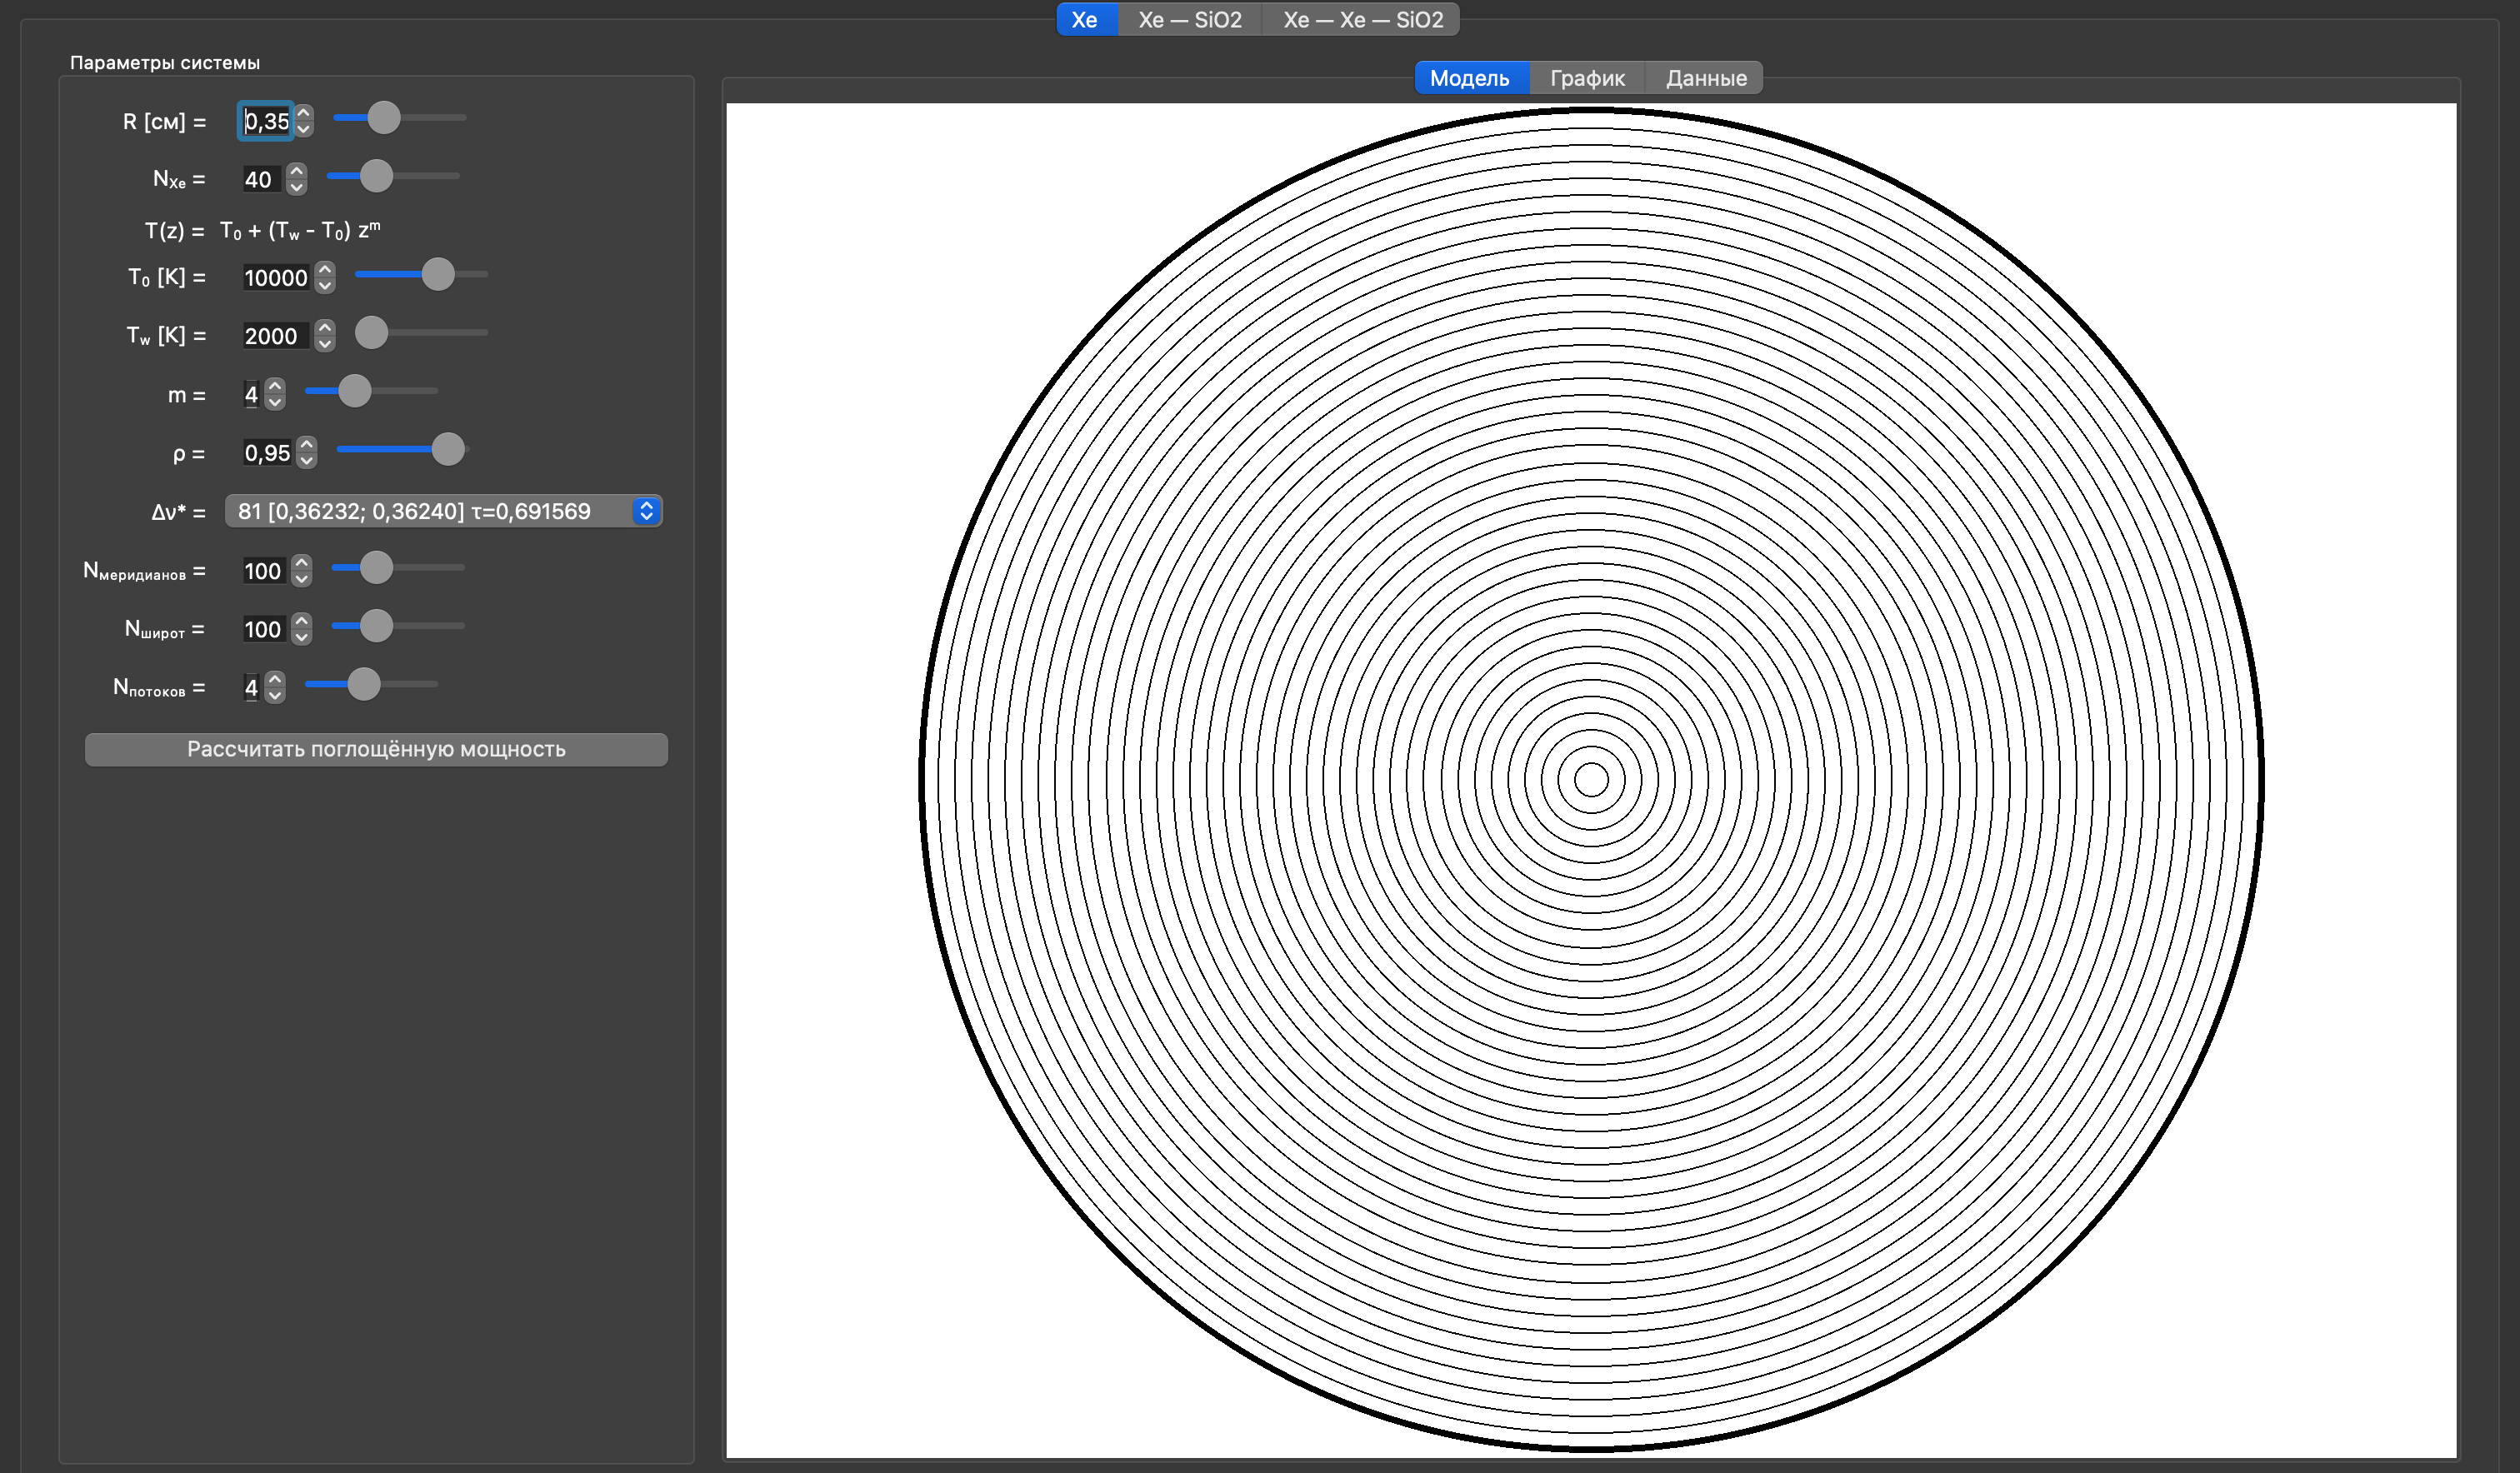
\includegraphics[width=\linewidth]{inc/img/tab-xe}
		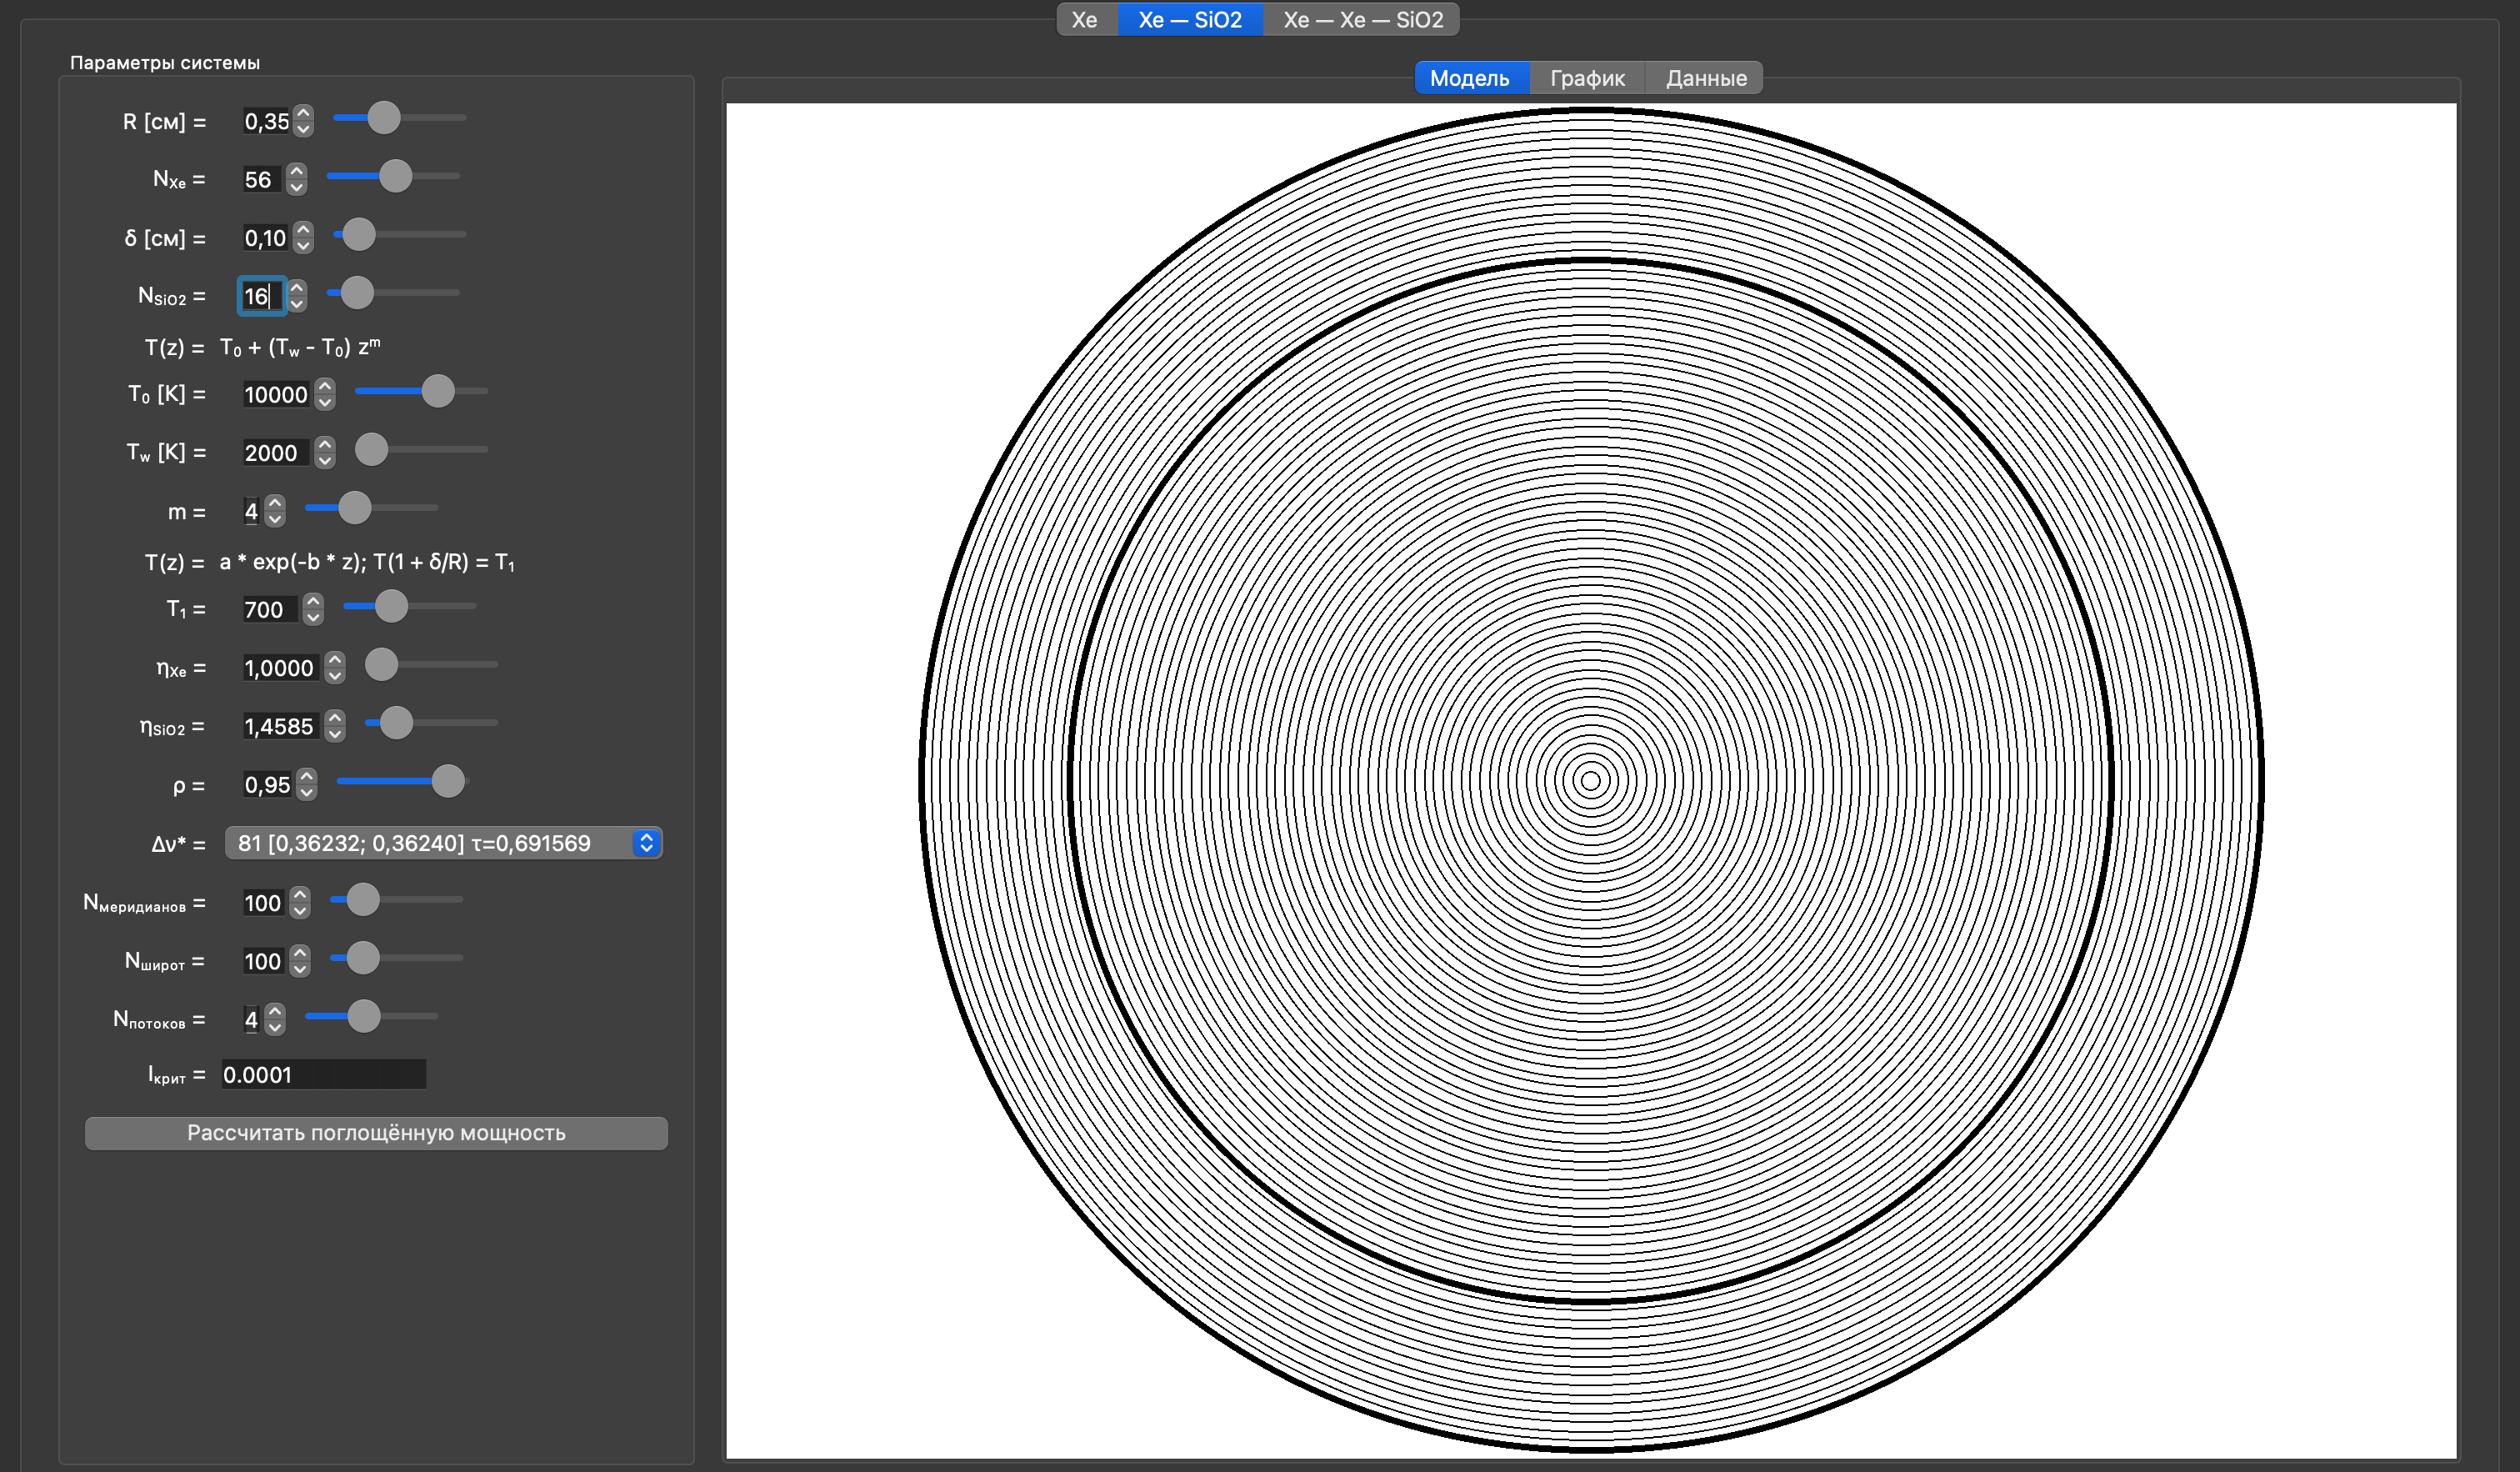
\includegraphics[width=\linewidth]{inc/img/tab-xe-sio2}
	}
	\captionsetup{justification=centering}
	\caption{Системы плазма~— отражатель и плазма~— оболочка~— отражатель}
	\label{img:xe-and-xe-sio2}
\end{figure}

%\imgh{width=\linewidth}{tab-xe}{tab-xe}
%\imgh{width=\linewidth}{tab-xe-sio2}{tab-xe-sio2}
\imgh{width=\linewidth}{tab-xe-xe-sio2}{Система плазма — оболочка — плазма — отражатель}

Входные параметры системы плазма — отражатель:
\begin{enumerate}
	\item $R$ [см] — радиус плазмы,
	\item $N_{Xe}$ — количество разбиений плазменного столба,
	\item $T_0$ [К] — осевая температура плазмы,
	\item $T_w$ [К] — радиальная температура плазмы,
	\item $m$ — показатель степени функции распределения температуры в плазме,
	\item $\rho$ — коэффициент отражения поверхности,
	\item $\Delta\nu^*$ — диапазон моделируемой частоты излучения,
	\item $N_{\text{меридианов}}$ — количество меридианов в сферическом излучении,
	\item $N_{\text{широт}}$ — количество широт,
	\item $N_{\text{потоков}}$ — количество потоков.
\end{enumerate}

Дополнительные входные параметры системы плазма~— оболочка~— отражатель:
\begin{enumerate}
	\item $\delta$ [см] — толщина оболочки,
	\item $N_{SiO2}$ — количество разбиений оболочки,
	\item $T_1$ [К] — радиальная температура оболочки,
	\item $\eta_{Xe}$ — коэффициент оптической плотности плазмы,
	\item $\eta_{SiO2}$ — коэффициент оптической плотности оболочки.
\end{enumerate}

Дополнительные входные параметры системы плазма~— оболочка~— плазма~— отражатель:
\begin{enumerate}
	\item $\delta$ [см] — расстояние от плазмы до центра оболочки,
	\item $a$ [см] — полудлина большой оси оболочки,
	\item $b$ [см] — полудлина малой оси оболочки.
\end{enumerate}

Выходные данные по результатам моделирования отображаются в трёх вкладках (рисунки \ref{img:tab-paint}~— \ref{img:tab-data}). $I$ [Вт/см$^2$] отражает удельную поглощённую мощность светового излучения, а $q_{s\nu}$ [Вт/см$^3$] — распределение поглощённой мощности по объёму:

\begin{equation}
	q_{s\nu} = \frac{2\pi I}{\langle r_{\text{цилиндра}} \rangle}.
\end{equation}

\imgh{width=\linewidth}{tab-paint}{Визуализация распределения поглощённой мощности по объёму}

\imgh{width=\linewidth}{tab-plot}{Графики распределения поглощённой мощности}

\imgh{width=\linewidth}{tab-data}{Численные результаты расчёта распределения поглощённой мощности}

\begin{FixLineStretch}
\section{Сборка ПО}
\end{FixLineStretch}

Сборка осуществляется системой CMake по сценарию, описанному в листинге \ref{lst:cmake}, где вместо \code{[options...]} можно использовать несколько ключей из следующего списка:
\begin{enumerate}
	\item \code{-DMT\_ENABLE\_CLANG\_TIDY=ON} — для активации статического анализатора кода при сборке проекта;
	\item \code{-DMT\_ENABLE\_COMPILER\_WARNINGS=ON} — для активации широкого набора стандартных предупреждений компилятора при сборке;
	\item \code{-DMT\_ENABLE\_IPO\_LTO=ON} — для активации оптимизаций времени компоновки;
	\item \code{-DMT\_ENABLE\_IWYU=ON} — для активации предупреждений о неоптимальных зависимостях заголовков при сборке;
	\item \code{-DMT\_ENABLE\_UNSAFE\_MATH\_OPTIMIZATIONS=ON} — для активации небезопасных агрессивных математических оптимизаций при сборке проекта;
	\item \code{-DMT\_USE\_DOUBLE=ON} — для использования чисел с плавающей запятой двойной точности;
	\item \code{-DCMAKE\_BUILD\_TYPE=Debug} — для сборки проекта в отладочном режиме;
	\item \code{-DCMAKE\_BUILD\_TYPE=Release} — для сборки проекта в релизном режиме;
	\item \code{-DCMAKE\_BUILD\_TYPE=RelWithDebInfo} — для сборки проекта в релизном режиме с отладочной информацией.
\end{enumerate}

% Компилятор должен поддерживать определённые ключевые особенности из стандарта C++ 20.
% Узнать, какие версии компиляторов поддерживают последний стандарт можно ознакомившись с информацией из источника \cite{cpp-compiler-support}.

\begin{lstlisting}[gobble=8, caption={Сборка\label{lst:cmake}}]
	mkdir build
	cd build
	cmake [options...] ..
	cmake --build . --target MT
	cmake --build . --target GUI
\end{lstlisting}

\begin{FixLineStretch}
\section{Модульное тестирование}
\end{FixLineStretch}

В листингах \ref{lst:cpp-unit-test-equation}—\ref{lst:cpp-unit-tests-intersection} представлены примеры модульных тестов основных функций моделирования траектории движения луча в световой системе на базе фреймворка GoogleTest.

\begin{lstlisting}[gobble=8, caption={Юнит-тест функции решения квадратных уравнений\label{lst:cpp-unit-test-equation}}]
	TEST(EquationTest, QuadraticEquationTwoRealSolutions) {
	  auto x0 = kZero;
	  auto x1 = kZero;

	  const auto result = equation::SolveQuadratic(5, 6, 1, x0, x1);

	  ASSERT_EQ(result, equation::Result::kHasRealSolution);
	  ASSERT_NEAR(x0, -1.0_F, kEps);
	  ASSERT_NEAR(x1, -0.2_F, kEps);
	}
\end{lstlisting}

\begin{lstlisting}[gobble=8, caption={Юнит-тест функции отражения\label{lst:cpp-unit-test-reflection}}]
	TEST(ReflectTest, ReflectRay45Degree) {
	  const auto incident = Vec3{1, -1, 0}.Normalized();
	  const auto normal = Vec3{0, -1, 0}.Normalized();
	  const auto expected = Vec3{1, 1, 0}.Normalized();

	  const auto reflected = Reflect(incident, normal);
	  ExpectVectorNear(reflected, expected);
	}
\end{lstlisting}

\pagebreak

\begin{lstlisting}[gobble=8, caption={Юнит-тест функции преломления\label{lst:cpp-unit-test-refraction}}]
	TEST(RefractTest, AirToGlass) {
	  const auto incident = Vec3{1, 1, -1}.Normalized();
	  const auto normal = Vec3{0, 0, -1}.Normalized();
	  constexpr auto kEtaI = 1.0_F;
	  constexpr auto kEtaT = 1.5_F;
	  constexpr auto kMu = kEtaI / kEtaT;
	  const auto z = std::sqrt(19) / 3;
	  const auto expected = Vec3{kMu, kMu, -z}.Normalized();

	  const auto refracted = Refract(incident, normal, kEtaI, kEtaT);
	  ExpectVectorNear(refracted, expected);
	}
\end{lstlisting}

\begin{lstlisting}[gobble=8, caption={Юнит-тест метода пересечения луча с поверхностью цилиндра\label{lst:cpp-unit-tests-intersection}}]
	TEST(CylinderZInfinite, IntersectX) {
	  const CylinderZInfinite cylinder{{}, 2};
	  constexpr Vec3 kPos{-10, 0, 0};
	  constexpr Vec3 kDir{1, 0, 0};
	  ASSERT_EQ(cylinder.Intersect(kPos, kDir), 8);
	}
\end{lstlisting}

\section*{Выводы}

В результате выполнения технологического раздела выпускной квалификационной работы разработано программно-математическое обеспечение, реализующее дискретно-лучевой метод моделирования световых полей в системах с неоднородными поглощающими и излучающими средами на основе параллельных вычислений.

Обоснованно выбран язык программирования, приведён список используемых технологий, представлена структура ПО, а также описаны: интерфейс приложения, входные/выходные данные, необходимая для сборки ПО информация и модульные тесты.
